\documentclass[11pt]{article}
%Gummi|063|=)
\title{\textbf{Algorithms I -- supervision 8}}
\author{James Wood}
\usepackage{listings}
\usepackage{bold-extra}
\usepackage{xcolor}
\usepackage{amsmath}
\usepackage{enumitem}
\usepackage{tikz}
\usetikzlibrary{arrows}

\lstset{
  basicstyle=\small,
  basewidth=0.5em,
  frame=single,
  breaklines=true,
  %postbreak=\raisebox{0ex}[0ex][0ex]{
  %  \ensuremath{\color{red}\hookrightarrow\space}
  %}
  language=python,
  literate=
    {<=}{{\(\leq\)}}1
    {>=}{{\(\geq\)}}1
    {&&}{{\(\wedge\)}}1
    {||}{{\(\vee\)}}1
    {->}{{\(\rightarrow\)}}1
}

\tikzset{
  treenode/.style = {align=center, inner sep=0pt, text centered,
    font=\sffamily},
  bnode/.style = {treenode, circle, white, draw=black,
    fill=black, text width=1.5em},
  rnode/.style = {treenode, circle, red, draw=red,
    text width=1.5em, very thick},
  leaf/.style = {treenode, rectangle, draw=black,
    minimum width=0.5em, minimum height=0.5em}
}

\begin{document}
\renewcommand{\labelenumi}{(\alph{enumi})}
\renewcommand{\labelenumii}{(\roman{enumii})}

\maketitle

\section{Graphs}
\begin{enumerate}
\item
  Start at a given vertex, assigning it a weight of 0, and add all edges leaving it to a priority queue ordered by the weight of the edge plus the weight of the vertex at their start (ascending). Remove edges from the queue until the taken edge ends at a vertex without an assigned weight. Give this vertex the weight stored as the key of the priority queue item and repeat the process until all vertices have been assigned a weight.

  Dijkstra's algorithm is a greedy algorithm, so chooses the route that minimises weight, under the assumption that worse paths cannot be made better by adding more edges. This assumption does not hold in a general graph with negative-weight edges.
\item
  A dummy vertex \(q\) is added to the graph, with edges going from it to each other vertex, each edge having weight 0. Then, the Bellman-Ford algorithm is run, starting at \(q\). From this, we obtain a function \(\delta:\mathrm{Vertex}\to\mathrm{Weight}\) describing how far the given vertex is away from \(q\). We then produce a new graph based on the original graph (with weight function \(w\)) with weight function \(w':\mathrm{Vertex}\times\mathrm{Vertex}\to\mathrm{Weight}\), where \(w'\,(u,v)=w\,(u,v)+\delta\,u-\delta\,v\). Since \(\delta\,v\leq\delta\,u+w\,(u,v)\), all edges in the new graph have positive weight. Hence, we can run Dijkstra's algorithm (which is quicker than Bellman-Ford) on each vertex.
\item
  Consider this graph:

  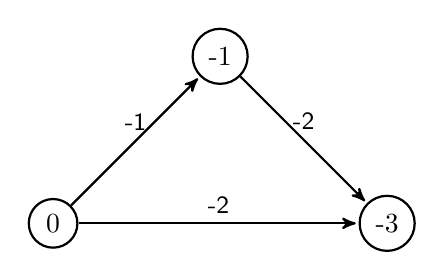
\begin{tikzpicture}[->,>=stealth',shorten >=1pt,auto,node distance=3cm,thick,main node/.style={circle,draw}]
    \node[main node] (0) {0};
    \node[main node] (1) [above right of=0] {-1};
    \node[main node] (2) [below right of=1] {-3};

    \path[every node/.style={font=\sffamily\small}]
    (0) edge node [above] {-1} (1)
    (1) edge node [above] {-2} (2)
    (0) edge node [above] {-2} (2);
  \end{tikzpicture}

  The shortest path from left to right goes via the middle node. Adding 2 to the weight of each arc gives this:

  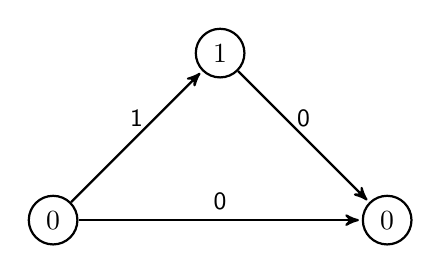
\begin{tikzpicture}[->,>=stealth',shorten >=1pt,auto,node distance=3cm,thick,main node/.style={circle,draw}]
    \node[main node] (0) {0};
    \node[main node] (1) [above right of=0] {1};
    \node[main node] (2) [below right of=1] {0};

    \path[every node/.style={font=\sffamily\small}]
    (0) edge node [above] {1} (1)
    (1) edge node [above] {0} (2)
    (0) edge node [above] {0} (2);
  \end{tikzpicture}

  The shortest path from left to right is now to go there directly. Hence, this tactic does not work.
\item
  A connected directed graph can be created such that certain notes are unreachable from others. In this case, starting from an existing node, in the worst case, won't assign weights to nodes, as needed for the reweighting of edges. Hence, Johnson's algorithm will fail.
\end{enumerate}

\section{DAG}
Starting in the top-left:

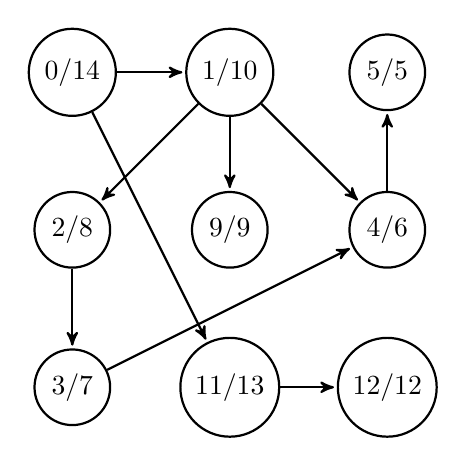
\begin{tikzpicture}[->,>=stealth',shorten >=1pt,auto,node distance=2cm,thick,main node/.style={circle,draw}]
  \node[main node] (0) {0/14};
  \node[main node] (1) [right of=0] {1/10};
  \node[main node] (2) [right of=1] {5/5};
  \node[main node] (3) [below of=0] {2/8};
  \node[main node] (4) [right of=3] {9/9};
  \node[main node] (5) [right of=4] {4/6};
  \node[main node] (6) [below of=3] {3/7};
  \node[main node] (7) [right of=6] {11/13};
  \node[main node] (8) [right of=7] {12/12};

  \path[every node/.style={font=\sffamily\small}]
  (0) edge (1)
  (0) edge (7)
  (1) edge (4)
  (7) edge (8)
  (6) edge (5)
  (1) edge (3)
  (3) edge (6)
  (5) edge (2)
  (1) edge (5);
\end{tikzpicture}

This gives (read left-to-right, then top-to-bottom):

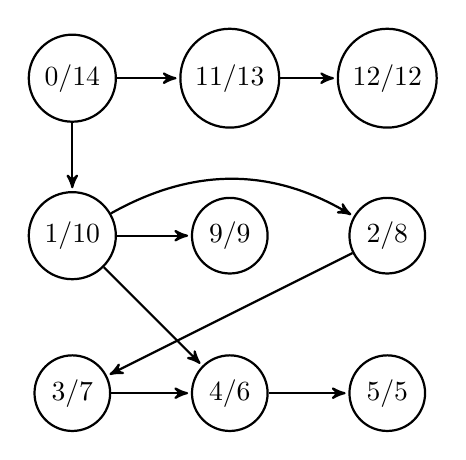
\begin{tikzpicture}[->,>=stealth',shorten >=1pt,auto,node distance=2cm,thick,main node/.style={circle,draw}]
  \node[main node] (0) {0/14};
  \node[main node] (7) [right of=0] {11/13};
  \node[main node] (8) [right of=7] {12/12};
  \node[main node] (1) [below of=0] {1/10};
  \node[main node] (4) [right of=1] {9/9};
  \node[main node] (3) [right of=4] {2/8};
  \node[main node] (6) [below of=1] {3/7};
  \node[main node] (5) [right of=6] {4/6};
  \node[main node] (2) [right of=5] {5/5};

  \path[every node/.style={font=\sffamily\small}]
  (0) edge (1)
  (0) edge (7)
  (1) edge (4)
  (7) edge (8)
  (6) edge (5)
  (1) edge [bend left] (3)
  (3) edge (6)
  (5) edge (2)
  (1) edge (5);
\end{tikzpicture}

And indeed, the arrows do go forward.

\section{Topological sort}
After a correctly computed topological sort, item A precedes item B if there is a path from A to B. After running the topological sort algorithm, A precedes B iff A's finish time is later than B's, according to a depth-first search. Hence, we are required to prove that if there is a path from A to B, A's finish time is later than B's. By definition, using the fact that A has children, A finishes once all of its children have finished. The child containing B (if B is not a child) will finish after B, and so on. Hence, A finishes after B, as required.

\section{Draw graphs}
\begin{enumerate}
\item
  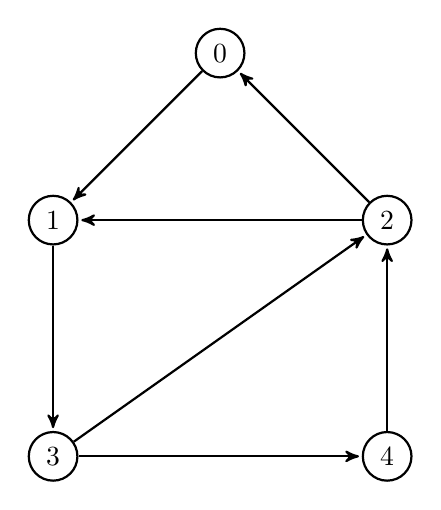
\begin{tikzpicture}[baseline={([yshift={-\ht\strutbox}]0.north)},->,>=stealth',shorten >=1pt,auto,node distance=3cm,thick,main node/.style={circle,draw}]
    \node[main node] (0) {0};
    \node[main node] (1) [below left of=0] {1};
    \node[main node] (2) [below right of=0] {2};
    \node[main node] (3) [below of=1] {3};
    \node[main node] (4) [below of=2] {4};

    \path[every node/.style={font=\sffamily\small}]
    (0) edge (1)
    (1) edge (3)
    (3) edge (4)
    (4) edge (2)
    (2) edge (0)
    (2) edge (1)
    (3) edge (2);
  \end{tikzpicture}
\item
  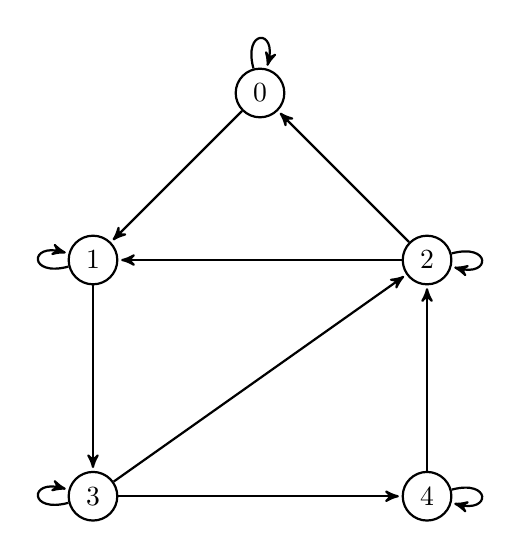
\begin{tikzpicture}[baseline={([yshift={-\ht\strutbox}]0.north)},->,>=stealth',shorten >=1pt,auto,node distance=3cm,thick,main node/.style={circle,draw}]
    \node[main node] (0) {0};
    \node[main node] (1) [below left of=0] {1};
    \node[main node] (2) [below right of=0] {2};
    \node[main node] (3) [below of=1] {3};
    \node[main node] (4) [below of=2] {4};

    \path[every node/.style={font=\sffamily\small}]
    (0) edge [loop above] (0)
    (1) edge [loop left] (1)
    (2) edge [loop right] (2)
    (3) edge [loop left] (3)
    (4) edge [loop right] (4)

    (0) edge (1)
    (1) edge (3)
    (3) edge (4)
    (4) edge (2)
    (2) edge (0)
    (2) edge (1)
    (3) edge (2);
  \end{tikzpicture}
\item
  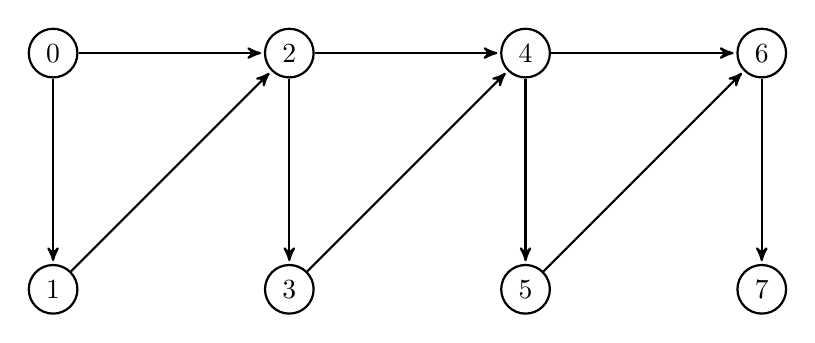
\begin{tikzpicture}[baseline={([yshift={-\ht\strutbox}]0.north)},->,>=stealth',shorten >=1pt,auto,node distance=3cm,thick,main node/.style={circle,draw}]
    \node[main node] (0) {0};
    \node[main node] (1) [below of=0] {1};
    \node[main node] (2) [right of=0] {2};
    \node[main node] (3) [right of=1] {3};
    \node[main node] (4) [right of=2] {4};
    \node[main node] (5) [right of=3] {5};
    \node[main node] (6) [right of=4] {6};
    \node[main node] (7) [right of=5] {7};

    \path[every node/.style={font=\sffamily\small}]
    (0) edge (1)
    (1) edge (2)
    (2) edge (3)
    (3) edge (4)
    (4) edge (5)
    (5) edge (6)
    (6) edge (7)
    (0) edge (2)
    (2) edge (4)
    (4) edge (6);
  \end{tikzpicture}
\item In a tree, \(|V|=|E|+1\).
\item A tree is defined as an undirected graph without cycles.
\item
  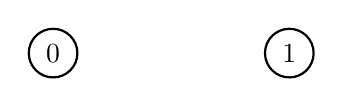
\begin{tikzpicture}[baseline={([yshift={-\ht\strutbox}]0.north)},->,>=stealth',shorten >=1pt,auto,node distance=3cm,thick,main node/.style={circle,draw}]
    \node[main node] (0) {0};
    \node[main node] (1) [right of=0] {1};
  \end{tikzpicture}
\end{enumerate}

\section{Matrices}
\begin{enumerate}
\item
  \(L^{(0)}=\begin{pmatrix} 0 & \infty & \hdots & \infty \\ \infty & 0 & \hdots & \infty \\ \vdots & \vdots & \ddots & \vdots \\ \infty & \infty & \hdots & 0 \end{pmatrix}\)
\item
  \(L^{(0)}\) acts like \(\begin{pmatrix} 1 & 0 & \hdots & 0 \\ 0 & 1 & \hdots & 0 \\ \vdots & \vdots & \ddots & \vdots \\ 0 & 0 & \hdots & 1 \end{pmatrix}\), the identity matrix.
\end{enumerate}

\section{Fibonacci heaps}
\begin{enumerate}
\item
  
\begin{tikzpicture}[baseline={([yshift={-\ht\strutbox}]0.north)},->,>=stealth',auto,node distance=1cm,thick,main node/.style={circle,draw}]
    \node[main node,double] (0) {18};
  \end{tikzpicture}

  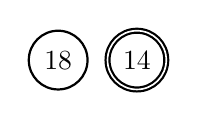
\begin{tikzpicture}[baseline={([yshift={-\ht\strutbox}]0.north)},->,>=stealth',auto,node distance=1cm,thick,main node/.style={circle,draw}]
    \node[main node] (0) {18};
    \node[main node,double] (1) [right of=0] {14};
  \end{tikzpicture}

  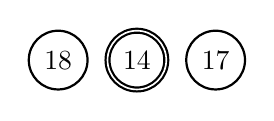
\begin{tikzpicture}[baseline={([yshift={-\ht\strutbox}]0.north)},->,>=stealth',auto,node distance=1cm,thick,main node/.style={circle,draw}]
    \node[main node] (0) {18};
    \node[main node,double] (1) [right of=0] {14};
    \node[main node] (2) [right of=1] {17};
  \end{tikzpicture}

  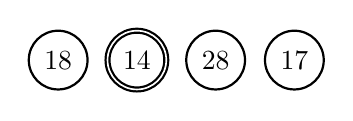
\begin{tikzpicture}[baseline={([yshift={-\ht\strutbox}]0.north)},->,>=stealth',auto,node distance=1cm,thick,main node/.style={circle,draw}]
    \node[main node] (0) {18};
    \node[main node,double] (1) [right of=0] {14};
    \node[main node] (3) [right of=1] {28};
    \node[main node] (2) [right of=3] {17};
  \end{tikzpicture}

  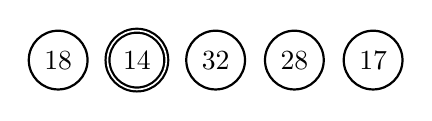
\begin{tikzpicture}[baseline={([yshift={-\ht\strutbox}]0.north)},->,>=stealth',auto,node distance=1cm,thick,main node/.style={circle,draw}]
    \node[main node] (0) {18};
    \node[main node,double] (1) [right of=0] {14};
    \node[main node] (4) [right of=1] {32};
    \node[main node] (3) [right of=4] {28};
    \node[main node] (2) [right of=3] {17};
  \end{tikzpicture}

  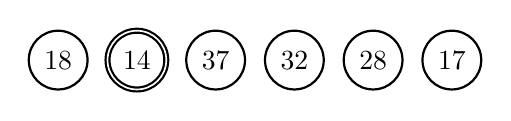
\begin{tikzpicture}[baseline={([yshift={-\ht\strutbox}]0.north)},->,>=stealth',auto,node distance=1cm,thick,main node/.style={circle,draw}]
    \node[main node] (0) {18};
    \node[main node,double] (1) [right of=0] {14};
    \node[main node] (5) [right of=1] {37};
    \node[main node] (4) [right of=5] {32};
    \node[main node] (3) [right of=4] {28};
    \node[main node] (2) [right of=3] {17};
  \end{tikzpicture}

  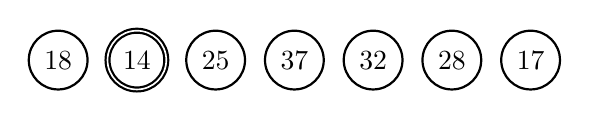
\begin{tikzpicture}[baseline={([yshift={-\ht\strutbox}]0.north)},->,>=stealth',auto,node distance=1cm,thick,main node/.style={circle,draw}]
    \node[main node] (0) {18};
    \node[main node,double] (1) [right of=0] {14};
    \node[main node] (6) [right of=1] {25};
    \node[main node] (5) [right of=6] {37};
    \node[main node] (4) [right of=5] {32};
    \node[main node] (3) [right of=4] {28};
    \node[main node] (2) [right of=3] {17};
  \end{tikzpicture}

  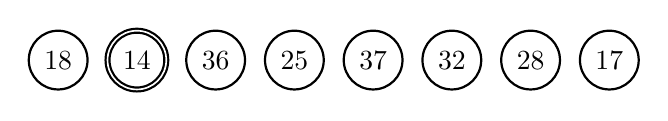
\begin{tikzpicture}[baseline={([yshift={-\ht\strutbox}]0.north)},->,>=stealth',auto,node distance=1cm,thick,main node/.style={circle,draw}]
    \node[main node] (0) {18};
    \node[main node,double] (1) [right of=0] {14};
    \node[main node] (7) [right of=1] {36};
    \node[main node] (6) [right of=7] {25};
    \node[main node] (5) [right of=6] {37};
    \node[main node] (4) [right of=5] {32};
    \node[main node] (3) [right of=4] {28};
    \node[main node] (2) [right of=3] {17};
  \end{tikzpicture}

  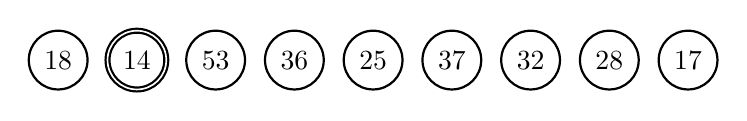
\begin{tikzpicture}[baseline={([yshift={-\ht\strutbox}]0.north)},->,>=stealth',auto,node distance=1cm,thick,main node/.style={circle,draw}]
    \node[main node] (0) {18};
    \node[main node,double] (1) [right of=0] {14};
    \node[main node] (8) [right of=1] {53};
    \node[main node] (7) [right of=8] {36};
    \node[main node] (6) [right of=7] {25};
    \node[main node] (5) [right of=6] {37};
    \node[main node] (4) [right of=5] {32};
    \node[main node] (3) [right of=4] {28};
    \node[main node] (2) [right of=3] {17};
  \end{tikzpicture}

  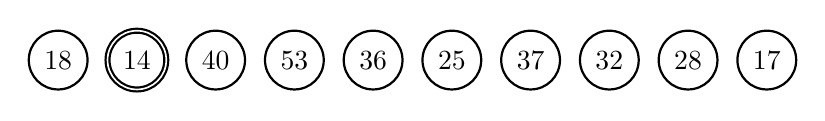
\begin{tikzpicture}[baseline={([yshift={-\ht\strutbox}]0.north)},->,>=stealth',auto,node distance=1cm,thick,main node/.style={circle,draw}]
    \node[main node] (0) {18};
    \node[main node,double] (1) [right of=0] {14};
    \node[main node] (9) [right of=1] {40};
    \node[main node] (8) [right of=9] {53};
    \node[main node] (7) [right of=8] {36};
    \node[main node] (6) [right of=7] {25};
    \node[main node] (5) [right of=6] {37};
    \node[main node] (4) [right of=5] {32};
    \node[main node] (3) [right of=4] {28};
    \node[main node] (2) [right of=3] {17};
  \end{tikzpicture}

  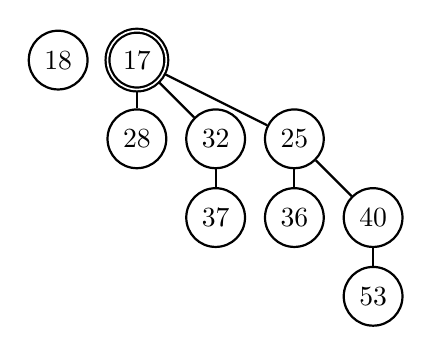
\begin{tikzpicture}[baseline={([yshift={-\ht\strutbox}]0.north)},>=stealth',auto,node distance=1cm,thick,main node/.style={circle,draw}]
    \node[main node] (0) {18};
    \node[main node,double] (2) [right of=0] {17};
    \node[main node] (3) [below of=2] {28};
    \node[main node] (4) [right of=3] {32};
    \node[main node] (5) [below of=4] {37};
    \node[main node] (6) [right of=4] {25};
    \node[main node] (7) [below of=6] {36};
    \node[main node] (9) [right of=7] {40};
    \node[main node] (8) [below of=9] {53};

    \path[every node/.style={font=\sffamily\small}]
    (2) edge (3)
        edge (4)
        edge (6)
    (4) edge (5)
    (6) edge (7)
        edge (9)
    (9) edge (8);
  \end{tikzpicture}

  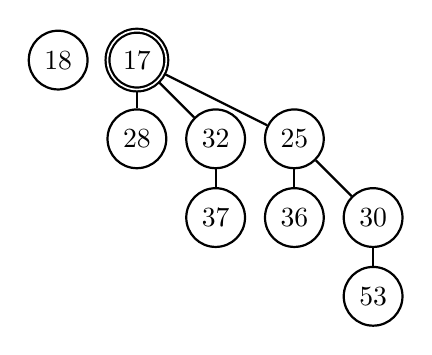
\begin{tikzpicture}[baseline={([yshift={-\ht\strutbox}]0.north)},>=stealth',auto,node distance=1cm,thick,main node/.style={circle,draw}]
    \node[main node] (0) {18};
    \node[main node,double] (2) [right of=0] {17};
    \node[main node] (3) [below of=2] {28};
    \node[main node] (4) [right of=3] {32};
    \node[main node] (5) [below of=4] {37};
    \node[main node] (6) [right of=4] {25};
    \node[main node] (7) [below of=6] {36};
    \node[main node] (9) [right of=7] {30};
    \node[main node] (8) [below of=9] {53};

    \path[every node/.style={font=\sffamily\small}]
    (2) edge (3)
        edge (4)
        edge (6)
    (4) edge (5)
    (6) edge (7)
        edge (9)
    (9) edge (8);
  \end{tikzpicture}

  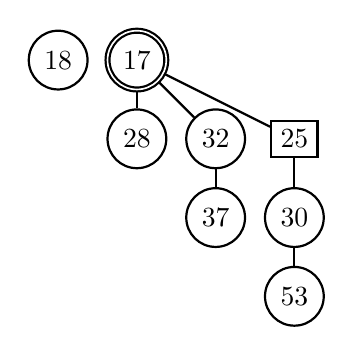
\begin{tikzpicture}[baseline={([yshift={-\ht\strutbox}]0.north)},>=stealth',auto,node distance=1cm,thick,main node/.style={circle,draw}]
    \node[main node] (0) {18};
    \node[main node,double] (2) [right of=0] {17};
    \node[main node] (3) [below of=2] {28};
    \node[main node] (4) [right of=3] {32};
    \node[main node] (5) [below of=4] {37};
    \node[main node,shape=rectangle] (6) [right of=4] {25};
    \node[main node] (9) [below of=6] {30};
    \node[main node] (8) [below of=9] {53};

    \path[every node/.style={font=\sffamily\small}]
    (2) edge (3)
        edge (4)
        edge (6)
    (4) edge (5)
    (6) edge (9)
    (9) edge (8);
  \end{tikzpicture}

  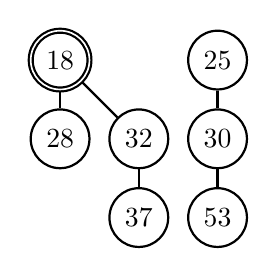
\begin{tikzpicture}[baseline={([yshift={-\ht\strutbox}]0.north)},>=stealth',auto,node distance=1cm,thick,main node/.style={circle,draw}]
    \node[main node,double] (0) {18};
    \node[main node] (3) [below of=0] {28};
    \node[main node] (4) [right of=3] {32};
    \node[main node] (5) [below of=4] {37};
    \node[main node] (9) [right of=4] {30};
    \node[main node] (6) [above of=9] {25};
    \node[main node] (8) [below of=9] {53};

    \path[every node/.style={font=\sffamily\small}]
    (0) edge (3)
        edge (4)
    (4) edge (5)
    (6) edge (9)
    (9) edge (8);
  \end{tikzpicture}
\item
  ?
\end{enumerate}

\end{document}